\documentclass[11pt, oneside]{article} 
\usepackage{geometry}
\geometry{letterpaper} 
\usepackage{graphicx}
	
\usepackage{amssymb}
\usepackage{amsmath}
\usepackage{parskip}
\usepackage{color}
\usepackage{hyperref}

\graphicspath{{/Users/telliott_admin/Tex/png/}}
% \begin{center} 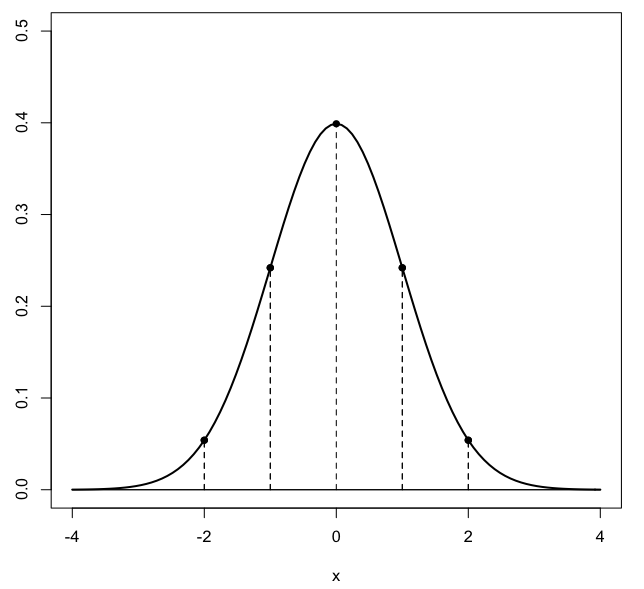
\includegraphics [scale=0.4] {gauss3.png} \end{center}

%break
\title{Determinants 1}
\date{}

\begin{document}
\maketitle
\Large

Strang says that all the usual properties of the determinant can be deduced from three simple rules.  \subsection*{1. $|I| =1$}
The determinant of the identity matrix $I$ equals $1$.
\[ 
|I| = 
\begin{vmatrix}
1  &  0 & 0 \\ 
0  &  1 & 0 \\
0 & 0 & 1  
 \end{vmatrix}
= 1
\]
\subsection*{2. row exchange may change the sign}
Each \emph{single} row exchange changes the sign of the determinant.  Some permutation matrices in $\mathbb{R}3$ are formed by two exchanges.
\[
\begin{vmatrix} 0  &  1 & 0 \\ 1  &  0 & 0 \\ 0 & 0  &  1 \end{vmatrix}
= -1, \ \ \ 
\begin{vmatrix} 0  &  0 & 1 \\ 1  &  0 & 0 \\ 0 & 1  &  0 \end{vmatrix}
= 1
\]
The rotation matrices in $\mathbb{R}2$ have determinant equal to $1$:
\[
\begin{vmatrix}
\cos \theta  &  -\sin \theta \\ 
\sin \theta  &  \ \ \cos \theta
 \end{vmatrix}
\]
as they do in $\mathbb{R}3$ 
\[
\begin{vmatrix}
1  &  0 & 0 \\ 
0  &  \cos \theta &  -\sin \theta \\ 
0 & \sin \theta & \ \ \cos \theta  
 \end{vmatrix}
 \]
\subsection*{3. linearity}
The determinant is a linear function of each row separately.
\[
\begin{vmatrix} ta & tb \\ c & d  \end{vmatrix}
= t
\begin{vmatrix} a & b \\ c & d  \end{vmatrix}
\]
For example 
\[
\begin{vmatrix} a  & 0 & 0 \\ 0  & b & 0 \\ 0 & 0 & c \end{vmatrix}
= abc
\]
and also
\[
\begin{vmatrix} a+a'  &  b+b' \\ c  &  d \end{vmatrix}
=
\begin{vmatrix} a  &  b \\ c  &  d \end{vmatrix}
+
\begin{vmatrix} a'  &  b' \\ c  &  d \end{vmatrix}
\]
Thus
\[ |A+B| = |A| + |B| \]

With those three rules, we can derive the rest.  Important rules:

\begin{itemize}
 \item row reduction operations do not change the determinant
 \item $A^{-1}$ exists $\iff |A| = 0$
 \item $|A| = |A^T|$
 \item $|AB| = |A| |B|$
 
\end{itemize}

To continue systematically:
\subsection*{4. equal rows}
If two rows of $\mathbf{A}$ are equal, $|\mathbf{A}| =0$.
\[
\begin{vmatrix} a & b \\ a & b \end{vmatrix}
= 0
\]
Proof:  exchange the two equal rows to give $\mathbf{A'}$.  Now, $|\mathbf{A}| = -|\mathbf{A'}|$ because of the exchange, but $|\mathbf{A}| = |\mathbf{A'}|$ because $\mathbf{A}=\mathbf{A'}$.  Therefore $|\mathbf{A}| = |\mathbf{A'}| = 0$.

\subsection*{5. no change with row reduction}
Row reduction methods don't change the determinant.
\[
\begin{vmatrix} a  &  b \\ c - ka &  d - kb \end{vmatrix}
=
\begin{vmatrix} a  &  b \\ c  &  d \end{vmatrix}
-
k
\begin{vmatrix} a  &  b \\ a  &  b \end{vmatrix}
\]

Proof:  the above is true by linearity (sequential application of rule 3).  But because of the equal rows in 
\[
-k
\begin{vmatrix} a  &  b \\ a  &  b \end{vmatrix}
\]
the second term is $0$ by rule 4, and thus, row reduction has not changed the determinant.

\subsection*{6. row of zeros}
If a matrix has a row of zeros, its determinant is equal to 0.
\[
\begin{vmatrix} a  &  b \\ 0 &  0 \end{vmatrix}
=
\begin{vmatrix} a  &  b \\ a  &  b \end{vmatrix}
\]
Proof:  use row reduction to add row 1 to row 2.  Now there are equal rows, so the determinant is equal to 0 (by rule 4).
\subsection*{7. triangular matrix}
A triangular matrix is one that looks like this

\[
\begin{bmatrix} 
d_1  &  a & b \\ 
0  &  d_2 & c \\ 
0 & 0  &  d_3
 \end{bmatrix}
 \]
called upper triangular, $U$, or alternatively the lower triangular matrix $L$
\[
\begin{bmatrix} 
d_1  &  0 & 0 \\ 
x  &  d_2 & 0 \\ 
y & z  &  d_3 
\end{bmatrix}
\]
In either case, we can use row reduction methods to zero out the off-diagonal entries without changing the entries along the diagonal.  Thus
\[
|U| = |L| = 
\begin{vmatrix} 
d_1  &  0 & 0 \\ 
0  &  d_2 & 0 \\ 
0 & 0  &  d_3 
\end{vmatrix}
\]
And those entries can be factored out to give
\[ d_1 d_2 d_3 |I |\]

Thus both $U$ and $L$ have determinant $d_1 \times d_2 \times d_3$.

\subsection*{8. singular matrix}
\[
|\mathbf{A}| = 0 \iff \mathbf{A} \text{ is \emph{singular}.}
\]
The determinant is zero if and only if the matrix is singular.  Proof:  produce $\mathbf{U}$ by row reduction methods, not changing the determinant.  If $\mathbf{U}$ is singular, it will have a zero row and $|\mathbf{U}| = 0$ by rule 6.  Otherwise, use rule 7.

\end{document}  